\documentclass[10pt, landscape]{article}
\usepackage[scaled=0.92]{helvet}
\usepackage{calc}
\usepackage{multicol}
\usepackage[a4paper,margin=3mm,landscape]{geometry}
\usepackage{amsmath,amsthm,amsfonts,amssymb}
\usepackage{color,graphicx,overpic}
\usepackage{hyperref}
\usepackage{newtxtext} 
\usepackage{enumitem}
\usepackage[table]{xcolor}
\usepackage{mathtools}
\setlist{nosep}
% for including images
\graphicspath{ {./images/} }

\pdfinfo{
  /Title (is2218_midterm_cheatsheet.pdf)
  /Creator (TeX)
  /Producer (pdfTeX 1.40.0)
  /Author (Gavin Chiam)
  /Subject (IS2218)
/Keywords (is2218, nus, cheatsheet, pdf)}

% Turn off header and footer
\pagestyle{empty}

% redefine section commands to use less space
\makeatletter
\renewcommand{\section}{\@startsection{section}{1}{0mm}%
  {-1ex plus -.5ex minus -.2ex}%
  {0.5ex plus .2ex}%x
{\normalfont\large\bfseries}}
\renewcommand{\subsection}{\@startsection{subsection}{2}{0mm}%
  {-1explus -.5ex minus -.2ex}%
  {0.5ex plus .2ex}%
{\normalfont\normalsize\bfseries}}
\renewcommand{\subsubsection}{\@startsection{subsubsection}{3}{0mm}%
  {-1ex plus -.5ex minus -.2ex}%
  {1ex plus .2ex}%
{\normalfont\small\bfseries}}%
\makeatother

\renewcommand{\familydefault}{\sfdefault}
\renewcommand\rmdefault{\sfdefault}
%  makes nested numbering (e.g. 1.1.1, 1.1.2, etc)
\renewcommand{\labelenumii}{\theenumii}
\renewcommand{\theenumii}{\theenumi.\arabic{enumii}.}
\renewcommand\labelitemii{•}
\renewcommand\labelitemiii{•}

\definecolor{mathblue}{cmyk}{1,.72,0,.38}
\everymath\expandafter{\the\everymath \color{mathblue}}

% Don't print section numbers
\setcounter{secnumdepth}{0}

\setlength{\parindent}{0pt}
\setlength{\parskip}{0pt plus 0.5ex}
%% adjust spacing for all itemize/enumerate
\setlength{\leftmargini}{0.4cm}
\setlength{\leftmarginii}{0.4cm}
\setlength{\leftmarginiii}{0.2cm}
\setlist[itemize,1]{leftmargin=2mm,labelindent=1mm,labelsep=1mm}
\setlist[itemize,2]{leftmargin=4mm,labelindent=1mm,labelsep=1mm}
\setlist[itemize,3]{leftmargin=4mm,labelindent=1mm,labelsep=1mm}

% adding my commands
\input{../commands/style-helpers.tex}
\makeatletter
\newcommand*{\xdashrightarrow}[2][]{%
  \mathrel{%
    \mathpalette{\da@xarrow{#1}{#2}{}\da@rightarrow{\,}{}}{}%
  }%
}
\newcommand*{\da@rightarrow}{\mathchar"0\hexnumber@\symAMSa 4B }
\newcommand*{\da@xarrow}[7]{%
  % #1: below
  % #2: above
  % #3: arrow left
  % #4: arrow right
  % #5: space left 
  % #6: space right
  % #7: math style 
  \sbox0{$\ifx#7\scriptstyle\scriptscriptstyle\else\scriptstyle\fi#5#1#6\m@th$}%
  \sbox2{$\ifx#7\scriptstyle\scriptscriptstyle\else\scriptstyle\fi#5#2#6\m@th$}%
  \sbox4{$#7\dabar@\m@th$}%
  \dimen@=\wd0 %
  \ifdim\wd2 >\dimen@
    \dimen@=\wd2 %   
  \fi
  \count@=2 %
  \def\da@bars{\dabar@\dabar@}%
  \@whiledim\count@\wd4<\dimen@\do{%
    \advance\count@\@ne
    \expandafter\def\expandafter\da@bars\expandafter{%
      \da@bars
      \dabar@ 
    }%
  }%  
  \mathrel{#3}%
  \mathrel{%   
    \mathop{\da@bars}\limits
    \ifx\\#1\\%
    \else
      _{\copy0}%
    \fi
    \ifx\\#2\\%
    \else
      ^{\copy2}%
    \fi
  }%   
  \mathrel{#4}%
}
\makeatother

% -----------------------------------------------------------------------

\begin{document}
\raggedright
\footnotesize
\begin{multicols*}{4}
  % multicol parameters
  \setlength{\columnseprule}{0.25pt}

  \begin{center}
    \fbox{%
      \parbox{0.8\linewidth}{\centering \textcolor{black}{
          {\Large\textbf{IS2218}}
        \\ \normalsize{AY25/26 SEM 1}}
        \\ {\footnotesize \textcolor{gray}{github/Gavino3o}}
      }%
    }
  \end{center}

  \section{Corp Governance and Agency Prob}

  \subsection{\underline{Investment vs Financing Decisions}}

  \begin{itemize}
    \item \textbf{Investment Decision}: How to allocate capital to long-term assets (tangible/intangible assets)
    \item Also known as \textbf{Capital Budgeting Decision} or \textbf{Capital Expenditure (CAPEX) Decision}
    \item Examples of investment decisions: launching a new product, expanding into a new market, acquiring another company, investing in research and development
    \item \textbf{Tangible assets}: physical assets used in operations.
    \item \textbf{Intangible assets}: non-physical assets that provide long-term value.
    \item Examples of tangible assets : machinery, buildings, land
    \item Examples of intangible assets: patents, trademarks, copyrights, goodwill
    \item \textbf{Real assets}: physical assets used in operations (e.g. machinery, buildings, land)
    \item \textbf{Financial assets}: financial instruments that represent a claim on future cash flows (e.g. stocks, bonds, derivatives)
  \end{itemize}

  \vspace{0.2cm}

  \begin{itemize}
    \item \textbf{Financing Decision}: How to raise capital to fund long-term investments
    \item Also known as \textbf{Capital Structure Decision}
    \item Mixture of debt and equity financing
    \item Debt financing: borrowing money from external sources (e.g. banks, bondholders) with the obligation to repay with interest
    \item Equity financing: issuing shares of stock to investors in exchange for ownership stake in the company
  \end{itemize}

  % \subsection{\underline{$Assets = Liabilities + Equity$}}

  % \begin{itemize}
  %   \item \textbf{Assets}: resources owned by the company that have economic value and can be used to generate future cash flows
  %   \item Real Assets: physical assets used in operations (e.g. machinery, buildings, land)
  %   \item Financial Assets: financial instruments that represent a claim on future cash flows (e.g. stocks, bonds, derivatives). These are also called \underline{securities}.
  %   \item \textbf{Liabilities}: obligations owed by the company to external parties that require future cash outflows
  %   \item Current Liabilities: obligations due within one year (e.g. accounts payable, short-term debt)
  %   \item Long-term Liabilities: obligations due beyond one year (e.g. long-term debt, bonds payable)
  %   \item \textbf{Equity}: residual interest in the assets of the company after deducting liabilities
  %   \item Common Stock: ownership shares in the company that represent a claim on future profits and voting rights
  %   \item Retained Earnings: accumulated profits that have been reinvested in the company rather than distributed to shareholders as dividends
  % \end{itemize}
  
  \subsection{\underline{Corporation}}

  \begin{itemize}
    \item A business organised as a separate legal entity owned by shareholders
    \item Shareholders elect a board of directors, who appoints managers to run the company and monitor their performance
    \item Sepearation of ownership and control. 
    \item (\textbf{Permanence}): Corporation continues to exist even if ownership changes
    \item (\textbf{Limited Liability}): The owners of a corporation are not personally liable for its obligations. Shareholders are only liable for the amount they invested in the company.
    \item \textbf{Types of Corporations}:
      \begin{itemize}
        \item \textbf{Public Corporation}: owned by a large number of shareholders and traded on public stock exchanges
        \item \textbf{Private Corporation}: owned by a small group of shareholders and not traded on public stock exchanges
      \end{itemize}
    \item \textbf{Types of Business Organisations}:
      \begin{itemize}
        \item \textbf{Sole Proprietorship}: owned and operated by a single individual
        \item \textbf{Partnership}: owned and operated by two or more individuals who share profits and losses
        \item \textbf{Corporation}: separate legal entity owned by shareholders
        \item \textbf{Limited Liability Company (LLC)}: hybrid structure that combines the benefits of a corporation and a partnership. No double taxation, limited liability, flexible management structure.
        \item \textbf{Professional Corporation (PC)}: for licensed professionals (e.g. doctors, lawyers, accountants). Limited liability for business debts, but not for professional malpractice (can be sued).
      \end{itemize}
      \vspace{0.2cm}

      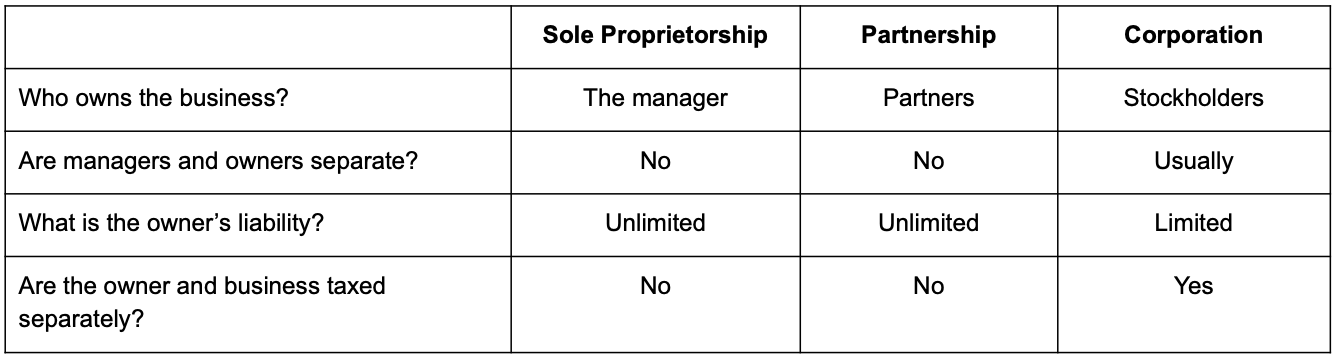
\includegraphics[width=0.97\linewidth]{corporation_table.png} 
  \end{itemize}

  \subsubsection{\underline{Financial Managers}}
  \begin{itemize}
    \item \textbf{Chief Financial Officer (CFO)}: oversees the financial operations/policies of the company and corporate planning
    \item \textbf{Treasurer}: manages the company's cash and investments, raises capital, and manages banking relationships
    \item \textbf{Controller}: oversees the accounting and financial reporting functions of the company, ensures compliance with financial regulations and standards
  \end{itemize}

  \subsection{\underline{Agency Problem}}
  \begin{itemize}
    \item \textbf{Goals of a Corporation:}
      \begin{itemize}
        \item Shareholders desire wealth maximization. Maximizing the current market value of shareholder's investment in the company.
        \item Why not profit maximization? Profit is a flow variable, while wealth is a stock variable. Profit does not account for the time value of money, risk, and cash flows. Earning manipulation to increase short-term profit may harm long-term wealth.
        \item \textbf{Opportunity cost of capital}: minimum acceptable rate of return on capital investments by shareholders (set by investment alternatives in the financial markets)
      \end{itemize}

    \item \textbf{Agency Problem}: conflict of interest between shareholders (principals) and managers (agents). Managers are agents of shareholders and are tempted to act in their own interests rather than maximizing shareholder value.
    \item Managers have constituencies called \textbf{stakeholders} (e.g. employees, customers, suppliers, creditors, government) whose interests may not align with shareholders.
    \item \textbf{Agency Costs:} Value lost from agency problems or from efforts to mitigate agency problems.
    \item \textbf{Solutions to Agency Problem:}
      \begin{itemize}
        \item \textbf{Executive Compensation}: align manager's interests with shareholders. E.g. stock options, bonuses tied to performance metrics (e.g. stock price, earnings per share)
        \item \textbf{Corporate Governance}: Systems of laws, regulations, policies, institutions, and corporate practices that protect shareholders and other investors.
        \item \textbf{Elements of Good Corporate Governance}:
          \begin{itemize}
            \item Legal requirements and regulations
            \item Board of Directors: independent directors, committees (e.g. audit, compensation, nomination)
            \item Activist shareholders: large shareholders who actively monitor and influence management
            \item Takeovers: threat of takeover can discipline management (e.g. If you share price is undervalued, another company may acquire you and replace management)
            \item Transparency and disclosure: accurate and timely financial reporting, disclosure of material information
          \end{itemize}
      \end{itemize}
  \end{itemize}

  \subsubsection{\underline{Ethics of Maximising Shareholder Wealth}}
  \begin{itemize}
    \item Short selling: selling borrowed shares in the hope of buying them back at a lower price to make a profit. (Can lead to market manipulation)
    \item Corporate raiders: investors who acquire a large stake in a company to influence management and increase shareholder value.
    \item Tax avoidance: legal strategies to minimize tax liability (e.g. offshore accounts, tax shelters)
  \end{itemize}

  \section{Platform Business Models}

  \begin{itemize}
    \item \textbf{Linear Value Chain:} traditional business model where value is created through a series of sequential activities \newline (e.g. Design $\rightarrow$ Manufacture $\rightarrow$ Sell $\rightarrow$ Deliver)
    \item \textbf{Platform Business Model:} business model that creates value by facilitating exchanges between two or more interdependent groups (e.g. buyers and sellers, users and developers) \newline (Producers $\rightarrow$ Platform $\leftarrow$ Consumers)
    \item Examples: Uber, Airbnb, Amazon, Facebook, Google
  \end{itemize}

  \subsubsection{\underline{Types of Platforms:}}
    \begin{itemize}
      \item \textbf{Product Platforms}: provide a foundation for creating and distributing products or services with improvments over time (e.g. iPhone, Tesla)
      \item \textbf{Transaction Platforms}: facilitate exchanges between buyers and sellers (e.g. eBay, Uber, Airbnb)
      \item \textbf{Innovation Platforms}: provide a foundation for third-party developers to create complementary products or services (e.g. iOS, Android, Windows)
      \item \textbf{Orthogonal Platforms}: Products or servies that are based on the sale of different services of two groups of customers who do not come into contact with each other (e.g. newspaper adverstising [client as a target], data brokers [client as a source])
      \item \textbf{Hybrid/Integrated Platforms}: combine elements of transaction and innovation platforms (e.g. Amazon, Google)
    \end{itemize}


    \subsubsection{\underline{Advantages of Platform Business Models:}}
      \begin{itemize}
        \item No gatekeepers: anyone can participate as a producer or consumer. Consumers have more choices and producers have access to a larger market.
        \item New sources of value and supply: Asset owning is not necessary. Expansion is less risky. Sharing economy (Optimising the use of idle assets)
        \item Community feedback loops: users can provide feedback and ratings, which can improve the quality of products and services.
        \item Focus has shifted from broadcast to segementation, and then to virality and social influence. 
        \item From push to pull: consumers have more control over what they consume and how they consume it.
        \item From outbound to inbound: consumers actively seek out products and services that meet their needs and preferences.
      \end{itemize}
      
    \subsection{\underline{Network Effects}}
    Network effects occur when the value of a platform increases or decreases for users as more participants join the platform. (Two-sided, different from price effects and brand effects)
    \begin{itemize}
      \item \textbf{Positive same side}: When the value of the platform increases for users on the same side as more users join (e.g. social networks like Facebook, where more friends joining increases the value for existing users).
      \item \textbf{Negative same side}: When the value of the platform decreases for users on the same side as more users join (e.g. congestion effects in ride-sharing platforms, where too many drivers can reduce earnings per driver).
      \item \textbf{Positive cross side}: When the value of the platform increases for users on one side as more users join the other side (e.g. more sellers on eBay attract more buyers, and vice versa).
      \item \textbf{Negative cross side}: When the value of the platform decreases for users on one side as more users join the other side (e.g. too many advertisers on a platform like YouTube can reduce the user experience for viewers due to excessive ads).
    \end{itemize}

    \subsubsection{\underline{Monetization}}
    \begin{itemize}
      \item Be careful with charging: Overcharging can drive users away, while undercharging can lead to unsustainable operations. Striking the right balance is crucial.
     \item Different types of platform monetization:
        \begin{itemize}
          \item \textbf{Transactional Fees}: Both buyers and sellers are not discouraged. Platforms should still provide other value added benefits to prevent users/producers taking the activity outside the platform
          \item \textbf{Access/Enhanced Access}: Charge producers for access to consumers or charge users for lowering barriers.
          \item \textbf{Enhanced Curation}: Improve quality of interactions of those who pay a premium. (e.g subscription for better vetting and screening of service providers)
        \end{itemize}

      \item \textbf{Important principles:}
        \begin{itemize}
          \item Avoid charging for value that users previously received for free.
          \item Avoid reducing access to value that users have become accustomed to receiving.
          \item Strive to create additional value that justifies the charge imposed.
          \item Monetization strategies should be considered when making initial platform design choices.
        \end{itemize}
    \end{itemize}

    \subsubsection{\underline{Metrics}}
    \begin{itemize}
      \item \textbf{Metrics for Traditional Pipeline Model:}
        \begin{itemize}
          \item Produce goods and services efficiently and sufficient for demand. (Operations)
          \item Reach customers through prpoer channels at appropriate prices. (Marketing)
          \item Generate adequate revenues to produce profits/value for investors (Finance)
          \item E.g. Cash flow, inventory turns, operating income, gross margin, overhead, ROI
        \end{itemize}

      \item \textit{Platforms generate value through network effects}
      \item \textbf{Rate of interaction success} and factors that contribute to it.
      \item Quantifying success in generating desirable interactions amongst participants.
      \item \textbf{Startup Phase:}
      \begin{itemize}
        \item Growth of active produces and consumers who are participating in large volumes of successful interactions
        \item \textbf{Liquidity}: The ease with which participants can find and engage with counterparties for successful interactions on the platform. (Active usage, active users $\div$ total users, new active users $\div$ total active users)
        \item \textbf{Matching Quality}: The degree to which the platform successfully connects participants with the right counterparties to fulfill their needs or preferences. (Percentage of search leading to interaction, correlation between interaction rate and long-term rate of activity)
        \item \textbf{Trust}: The level of confidence participants have in the platform and its participants to ensure fair and reliable interactions. (Review system)
        \item \textit{Outcome based metrics, Metrics measuring commitment to ecosystem, Content creation metrics, Market access regardless of complete interaction}
      \end{itemize}

      \item \textbf{Growth Phase:}
      \begin{itemize}
        \item \textbf{Balance}: The platform's ability to maintain an appropriate ratio of producers to consumers to ensure a healthy ecosystem. (E.g. producer-to-consumer ratio, interaction success rate across different user groups)
        \item \textbf{Side Switching Rate}: The frequency with which users switch roles between producers and consumers on the platform. (E.g. percentage of users who act as both producers and consumers within a given time period)
        \item \textbf{Producer Side}
        \begin{itemize}
          \item Frequency of producer participation, listings created, outcomes achieved
          \item Interaction failure (initiated interactions that fall through)
          \item Producer fraud (Failure to describe product offering accurately or deliver product)
          \item Retention and Lifetime Value: Metrics that measure the ability of the platform to retain users over time and the long-term value generated by each user. (E.g. customer retention rate, average customer lifetime value, churn rate[lower the better])
        \end{itemize}
        \item \textbf{Consumer Side Side:}
          \begin{itemize}
            \item Frequency of consumption, searches, and rate of conversion to sale.
            \item Retention and Lifetime Value metrics as in a traditional business.
          \end{itemize}
      \end{itemize}

      \item \textbf{Maturity Phase:}
        \begin{itemize}
          \item Driving innovation: platform must adapt to the needs of its users and changes in competive and regulatory environment.
          \item E.g Incorporate third-party feature that provides a large share of value enjoyed by users as own feature.
        \end{itemize}
    \end{itemize}

    \subsubsection{\underline{Future of Platform Revolution}}
    \begin{itemize}
      \item \textbf{Joinining the revolution:} Information intensive industries; Industries with non-scalable gatekeepers; Highly fragmented industries (market aggregation); Industries characterised by extreme information assymetries.
      \item \textbf{Resist disruption:} Industries with high regulatory control, Industries with high failure costs (patient-doctor); Resource intensive industries
    \end{itemize}

    \section{Accounting Essentials}
    \textbf{Balance Sheet} \newline
    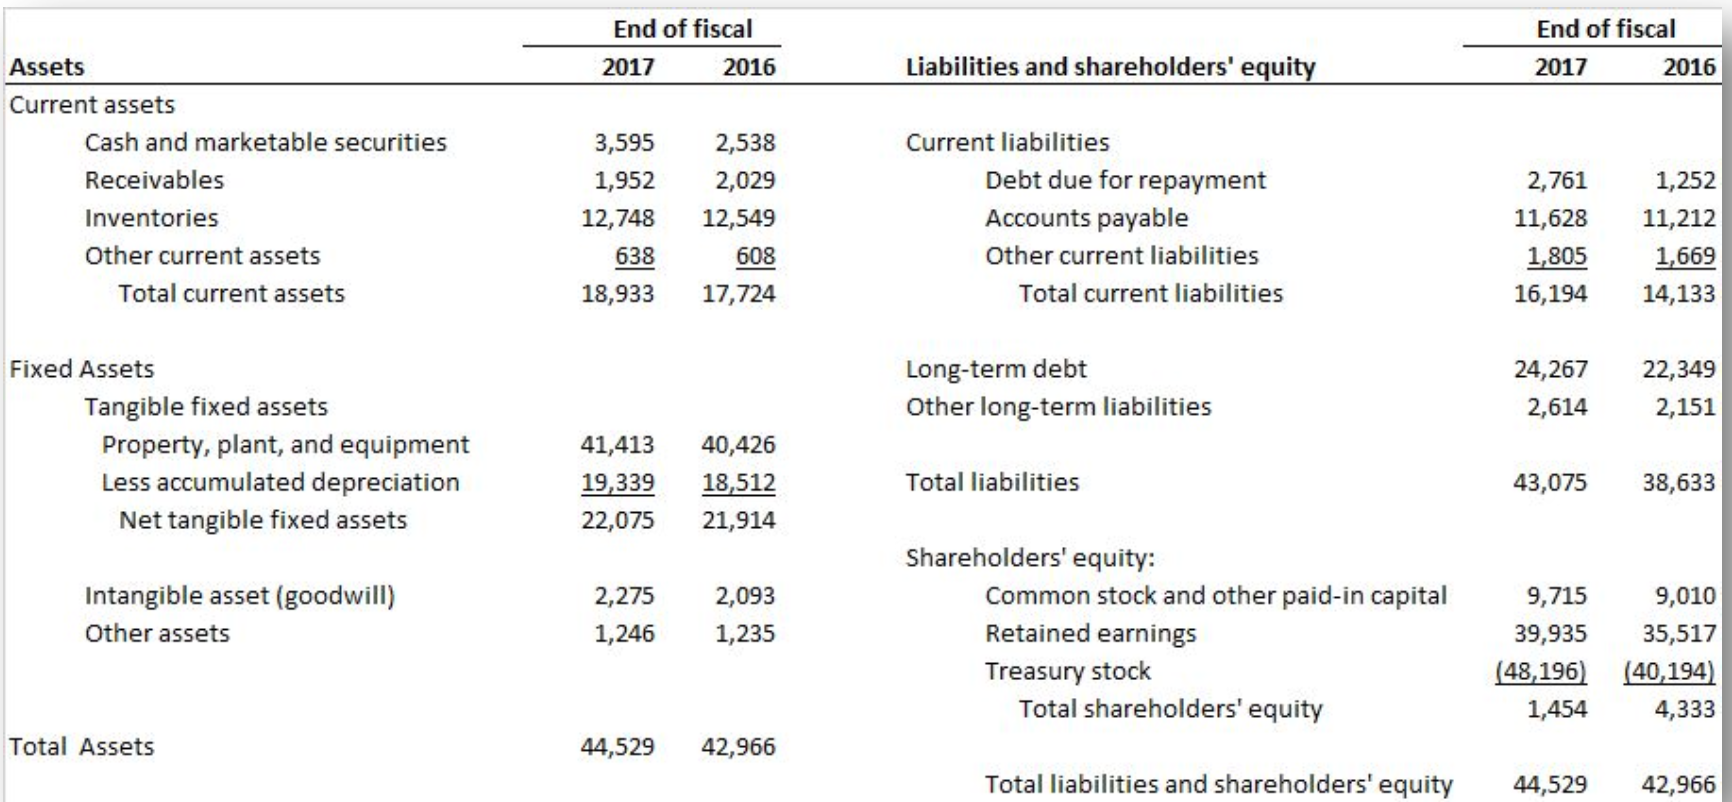
\includegraphics[width=0.97\linewidth]{balance_sheet_example.png}
    \textbf{Income Statement} \newline
    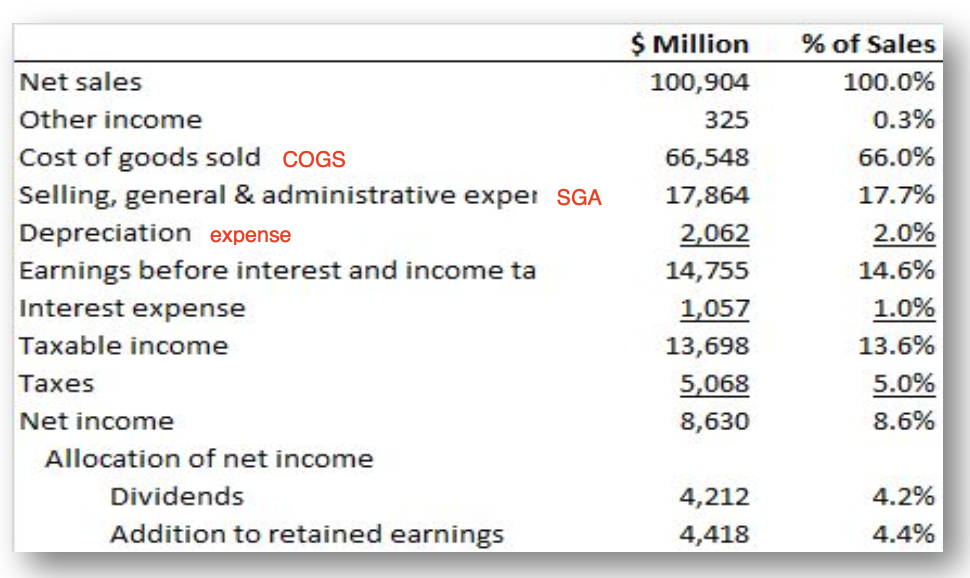
\includegraphics[width=0.97\linewidth, height=3cm]{income_statement_example.png}
    \textbf{Statement of Cash Flow} \newline
    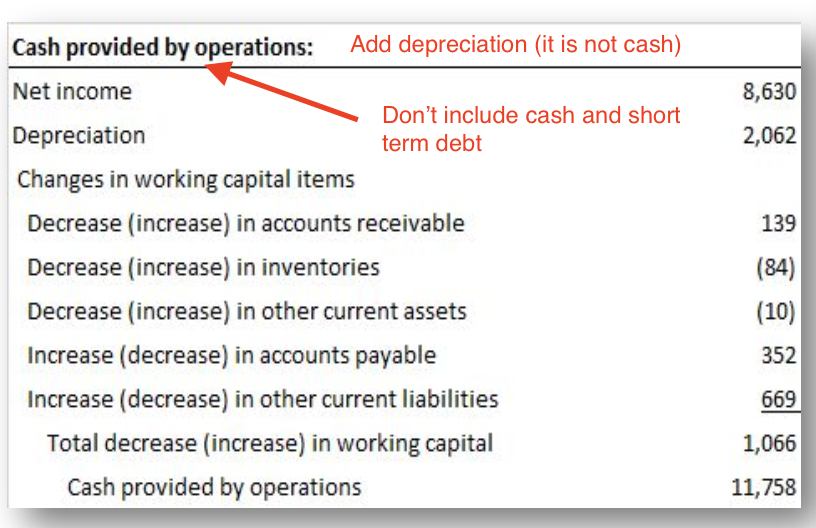
\includegraphics[width=0.97\linewidth, height=3cm]{cash_flow_1.png}
    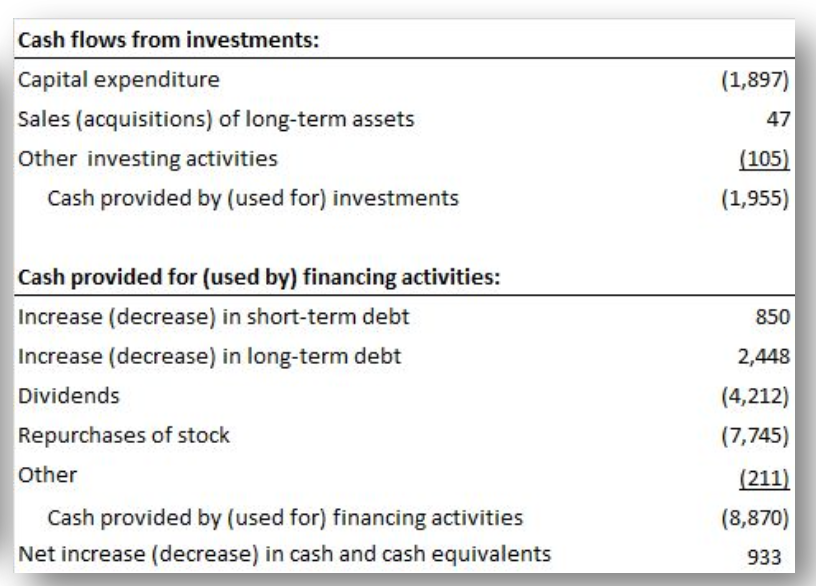
\includegraphics[width=0.97\linewidth, height=4cm]{cash_flow_2.png}
    \begin{itemize}
      \item Asset Decrease $\rightarrow$ Cash Inflow
      \item Asset Increase $\rightarrow$ Cash Outflow
      \item Liability Increase $\rightarrow$ Cash Inflow
      \item Liability Decrease $\rightarrow$ Cash Outflow
    \end{itemize}
    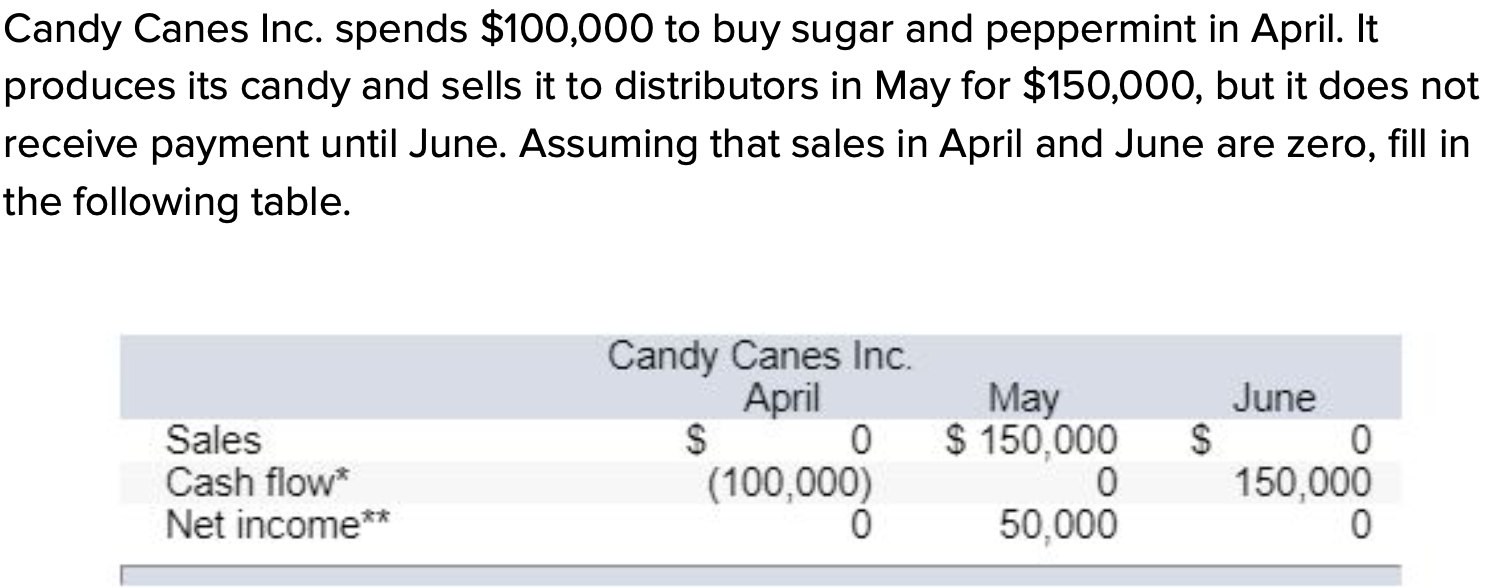
\includegraphics[width=0.8\linewidth, height=3cm]{cash_flow_example.png}


    
    \subsubsection{\underline{Notes}}

    \begin{itemize}
      \item \textbf{Interest expense (from loans) is tax exempt}. If the company is fully financed by equity, the tax shield benefit of debt financing is not utilized, potentially leading to higher overall tax liabilities.
      \item If the firm has Net Operating Loss (negative taxable income), it can carry forward the loss to offset taxable income in future years, reducing future tax liabilities. This is known as a \textbf{tax loss carryforward}. For example:
      \begin{itemize}
        \item A company incurs a net operating loss of \$100,000 in Year 1.
        \item In Year 2, the company generates a taxable income of \$150,000.
        \item The tax loss carryforward allows the company to offset the Year 2 taxable income with the Year 1 loss, reducing the taxable income to \$50,000.
        \item This results in lower taxes for Year 2, as the company only pays taxes on \$50,000 instead of \$150,000.
      \end{itemize}
      \item \textbf{Marginal tax rate:} highest tax rate a taxpayer encounters
    \end{itemize}

    \subsubsection{\underline{Equations}}
    \begin{itemize}
      \item assets = liability + equity
      \item equity = common stock + treasury stock + retained earnings
      \item networking capital = current assets - current liabilities
      \item EBIT = total revenue + other income - COGS - depreciation
      \item taxable income = EBIT - interest expense
      \item net income = taxable income - taxes
      \item taxes = taxable income $\times$ tax rate
      \item retained earnings = net income - dividends
      \item net increase (decrease) in cash and equivalents = cash operations $\pm$ cash investments $\pm$ cash financing activities
      \item free cash flow = net income + interest + depreciation - additions to networking capital + cashflow from investments
      \item free cash flow = interest + cashflow from operations + cashflow from investments (aka capital expenditure)
    \end{itemize}
    
\end{multicols*}

\end{document}
